% Copyright 2026 Sreeram Anil
% SPDX-License-Identifier: CC-BY-4.0
\chapter{Pack-level results}
\label{ch:res-pack}

\section{The module benchmark}

The pack benchmark (\cref{sec:ds-pack}) runs seven estimators on a twelve-cell series module
over the eVTOL mission, six scenarios and three seeds. Every cell is an independent
equivalent-circuit plant with its own capacity, impedance, initial SOC and ambient temperature
drawn from a manufacturing spread, all cells share one current sensor, and each has its own
voltage channel. The estimators are handed the same nominal parameter set for every cell. The
three decentralised references run one full filter per cell (EKF, UKF or reduced-order EKF)
with no exchange of information; the bar--delta filter runs one full filter on the module-average cell and
twelve small deviation filters (SOC deviation and relative impedance deviation) at a reduced
rate; the federated and
information-fusion filters run twelve local filters and fuse them through a master; and the
consensus filter lets neighbouring cells exchange information estimates over a ring.
\Cref{tab:pack_overview} gives the per-cell SOC RMSE over all cells (\cref{eq:me-pack-cells}),
the cost per pack step, the state memory and the number of scalars exchanged per step;
\cref{fig:res-pack} plots the same numbers.

% Copyright 2026 Sreeram Anil
% SPDX-License-Identifier: CC-BY-4.0
\begin{table}[H]\centering\footnotesize\setlength{\tabcolsep}{3pt}\caption{Pack-level overview: per-cell SOC RMSE [\%] by scenario (mean over seeds), cost per pack step and communication load.}\label{tab:pack_overview}
\begin{tabular}{lrrrrrrrrr}\toprule estimator & \rotatebox{60}{nominal} & \rotatebox{60}{init\_error} & \rotatebox{60}{current\_bias} & \rotatebox{60}{weak\_cell} & \rotatebox{60}{noise\_step} & \rotatebox{60}{large\_imbalance} & µs/step & kB & msgs \\ \midrule
Decentralized-EKF & 1.23 & 1.18 & 1.37 & 1.29 & 1.22 & 1.74 & 5.7 & 52.0 & 0 \\
BarDelta & 0.59 & 0.64 & 0.84 & 0.67 & 0.61 & 1.22 & 0.8 & 5.6 & 12 \\
Federated & 0.55 & 0.54 & 0.84 & 0.57 & 0.56 & 0.94 & 8.3 & 53.5 & 183 \\
Consensus & 0.66 & 0.63 & 0.79 & 0.64 & 0.69 & 1.39 & 9.3 & 9.2 & 216 \\
InfoFusion & 0.55 & 0.54 & 0.84 & 0.57 & 0.56 & 0.94 & 1.9 & 5.5 & 12 \\
Decentralized-UKF & 1.41 & 1.67 & 1.50 & 2.34 & 1.42 & 1.90 & 16.8 & 57.3 & 0 \\
Decentralized-ReducedEKF & 1.81 & 1.81 & 1.89 & 2.46 & 1.81 & 1.83 & 4.2 & 51.3 & 0 \\
\bottomrule\end{tabular}\end{table}


\begin{figure}[H]\centering
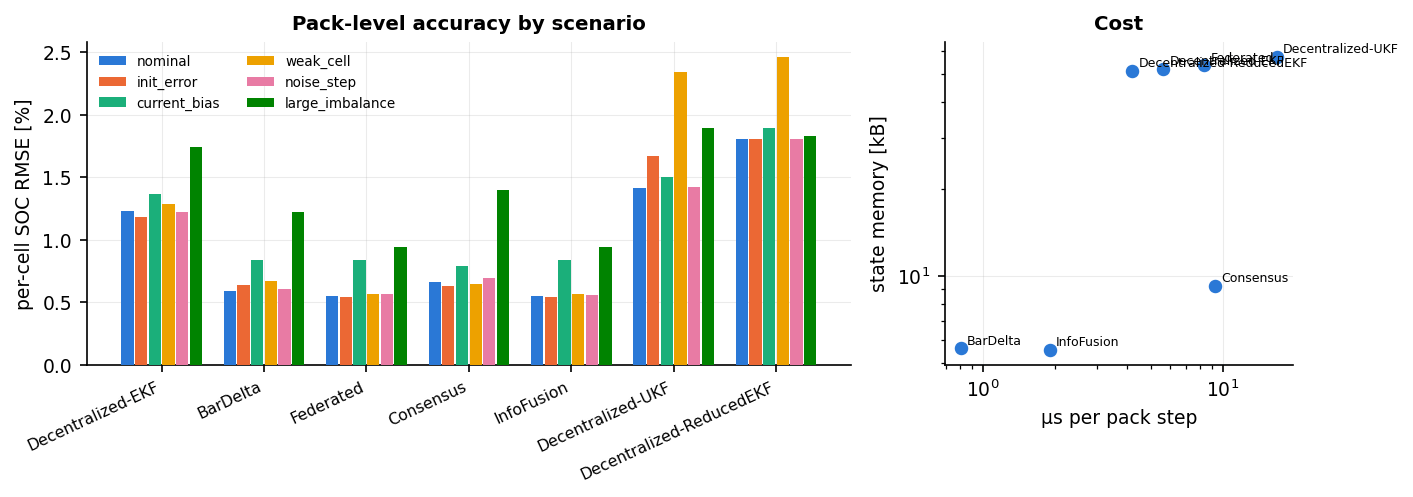
\includegraphics[width=\textwidth]{figures/pack_overview.png}
\caption{Pack-level accuracy by scenario (left) and cost (right). The two architectures that
average the twelve voltage channels inside the filter --- bar--delta and information fusion ---
halve the error of the decentralised EKF at a seventh and a third of its cost.}
\label{fig:res-pack}
\end{figure}

\section{What the numbers say}

\paragraph{Averaging is the whole story.} The decentralised EKF reaches \SI{1.23}{\percent} per
cell on the nominal module, twenty-five times its single-cell nominal figure. The difference is
the parameter spread: each cell's filter runs with resistances that are on average
\SI{8}{\percent} wrong and a capacity \SI{2}{\percent} wrong, which is the single-cell
\code{param\_mismatch} situation, and the per-cell error settles at the same
\num{1.2}--\num{1.4}\,\% as that scenario. The \emph{mean} of the twelve estimates, however, is
accurate to \SI{0.42}{\percent} (\cref{eq:me-pack-mean}), because the twelve voltage channels
carry independent noise and independent parameter errors that cancel in the average. The four
pack-level architectures do that averaging inside the filter instead of after it, and every one
of them halves the per-cell error: federated and information fusion \SI{0.55}{\percent},
bar--delta \SI{0.59}{\percent}, consensus \SI{0.66}{\percent}. The improvement is uniform across
\code{nominal}, \code{init\_error} and \code{noise\_step}, and it holds for the weakest-cell
estimate that determines the usable discharge (\cref{eq:me-pack-min}): \SI{0.48}{\percent}
for information fusion and \SI{0.56}{\percent} for bar--delta against \SI{0.81}{\percent} for
the decentralised EKF.

\paragraph{The common-mode current fault is not averaged away.} A \SI{0.25}{\ampere} bias with
a \SI{2}{\percent} gain error on the shared current sensor is the same error in every cell's
Coulomb count, and no amount of exchange between cells can separate it from the truth; all
seven estimators read \num{0.79}--\num{1.9}\,\% on \code{current\_bias}, and the four pack
architectures are within \num{0.05} points of each other at \num{0.79}--\num{0.84}. The pack
problem inherits the single-cell conclusion of \cref{ch:res-cell_ecm}: a current-sensor bias is
handled by calibrating the sensor, not by the estimator.

\paragraph{The weak cell is found by the estimator that has a state for it.} In
\code{weak\_cell} cell~5 has \SI{12}{\percent} less capacity and \SI{30}{\percent} more
resistance than the nominal set. The decentralised filters track it with their usual floor
(EKF \SI{1.29}{\percent} on the weakest cell), the bar--delta filter, whose delta-capacity states
identify the cell explicitly, with \SI{0.56}{\percent}, information fusion and federated with
\SI{0.51}{\percent}. The decentralised UKF and reduced-order EKF, on the other hand, lose the
weak cell entirely --- \num{5.65} and \SI{5.53}{\percent} on the weakest-cell estimate, with
maximum per-cell errors of \num{13} and \SI{21}{\percent} --- for two different reasons: a cell that drifts \num{0.10} away from the
trajectory on which the sigma points were seeded exposes the subtractive covariance update of
the unscented transform, and the reduced-order model has no state left in which to absorb a
\SI{30}{\percent} resistance error; \cref{ch:decentralizedukf,ch:decentralizedreducedekf}
document both.

\paragraph{Imbalance costs everyone, and the mean is not the answer.} With an initial SOC
spread of \num{0.05} and a \SI{5}{\percent} capacity spread (\code{large\_imbalance}) every
estimator is worse, the pack architectures by \SIrange{0.4}{0.7}{} points and the decentralised
EKF by \num{0.5}. The weakest-cell estimate now carries \num{1.65}--\num{2.45}\,\% for every
method, which is the practical statement that the usable-discharge SOC of an unbalanced module
is known to about two percent by any of these estimators --- and that a module in this
condition needs balancing before it needs a better estimator.

\paragraph{Cost.} The four pack architectures differ by an order of magnitude in what they
spend for the same accuracy. Information fusion and bar--delta run a pack step in \num{1.9}
and \SI{0.8}{\micro\second} with \SI{5.5}{} and \SI{5.6}{\kilo\byte} of state and twelve
scalars exchanged per step; the federated filter reaches the identical result --- to the digit,
because the two are algebraically the same fusion with different bookkeeping --- at
\SI{8.3}{\micro\second}, \SI{53.5}{\kilo\byte} and 183 scalars; the consensus filter, whose
ring exchange is what a distributed slave-board architecture would actually implement, costs
\SI{9.3}{\micro\second} and 216 scalars per step for \SI{0.66}{\percent}. The decentralised EKF
costs \SI{5.7}{\micro\second} for twelve full filters, i.e.\ the single-cell EKF times twelve.

\section{What the pack results say}

For a series module with one current sensor and per-cell voltage sensing, the estimator
architecture matters more than the estimator: the bar--delta filter, which is one EKF on the
average cell plus twelve two-state deviation filters, is twice as accurate as twelve independent EKFs and
seven times cheaper, and the information-fusion filter gives the same accuracy for a third
of the decentralised cost. The consensus filter is the choice when the cells are monitored
by separate slave boards with a serial bus between them, and pays for that in bus traffic.
The decentralised architecture keeps its place where the cells do \emph{not} share a current
(parallel groups) and where fault isolation between channels is a requirement, and in that
case the plain EKF is the right per-cell filter: the sigma-point and reduced-order variants
bring nothing at the module level and fail the weak-cell case. Balancing, not estimation, is
the remedy for a module with a large SOC spread.
